\documentclass[../report_polarFIR.tex]{subfiles}
\begin{document}
\chapter{CORDIC}

The next unit in the processing chain, as shown in Figure \ref{processingChainGraph}, is the CORDIC rotational computer. The CORDIC is implemented in Vitis HLS using equations shown in section \ref{cordicTheory}. The CORDIC's inputs are specified on a range generated by the worst-case scenario of the FIR filter's behavior, which is $\pm 125000$ given an input to the FIR of $\pm 50$ (refer to section \ref{FIRdata}). Additionally the FIR filter outputs data in a cartesian $(x, y)$ form. The CORDIC recieves these vectors of the cartesian form 
\begin{equation}
	d = \alpha + j\beta
\end{equation}
and converts them into polar form
\begin{equation}
	d = (r, \theta)
\end{equation}
where
\begin{equation}
	r = \sqrt{a^2 + b^2}
\end{equation}
and
\begin{equation}
	\theta = \tan^{-1}\left({\frac{\beta}{\alpha}}\right)
\end{equation}

As discussed in section \ref{cordicTheory}, this calculation is not trivial. However, it is possible to translate the coordinate system shift into the algorithm seen below in Listing \ref{CORDICalgo}.

		\begin{singlespace}
            \lstinputlisting[breaklines=true,
            label={CORDICalgo},
            caption={CORDIC algorithm},
            style=c-style,
            language=C++,
            firstnumber=1,
            linerange={112-161},
            ]{../source/CORDIC.cpp}
        \end{singlespace}

Analysis of this algorithm shows that it is an iterative process that over/under rotates the vector at decrementing amounts until the target angle has been reached. The actual rotation of the vectors is accomplished via simple multiplication of a matrix, shown in equations \ref{CORDICxCalc} and \ref{CORDICyCalc}. 



\section{Performance of the CORDIC}

The performance of the CORDIC leverages three 



One critical parameter of the algorithm is the number of iterations, or rotations, to perform. A method to estimate the convergence of the CORDIC algorithm is to inspect the CORDIC gain coefficents calculated using equation \ref{gainEQ}. The inverse of these coefficients ($K_i ^{-1}$) can be plotted to show convergence of the coefficients, as shown in Figure \ref{CORDICcoeffPlot}.

\begin{figure}[h!]
\begin{center}
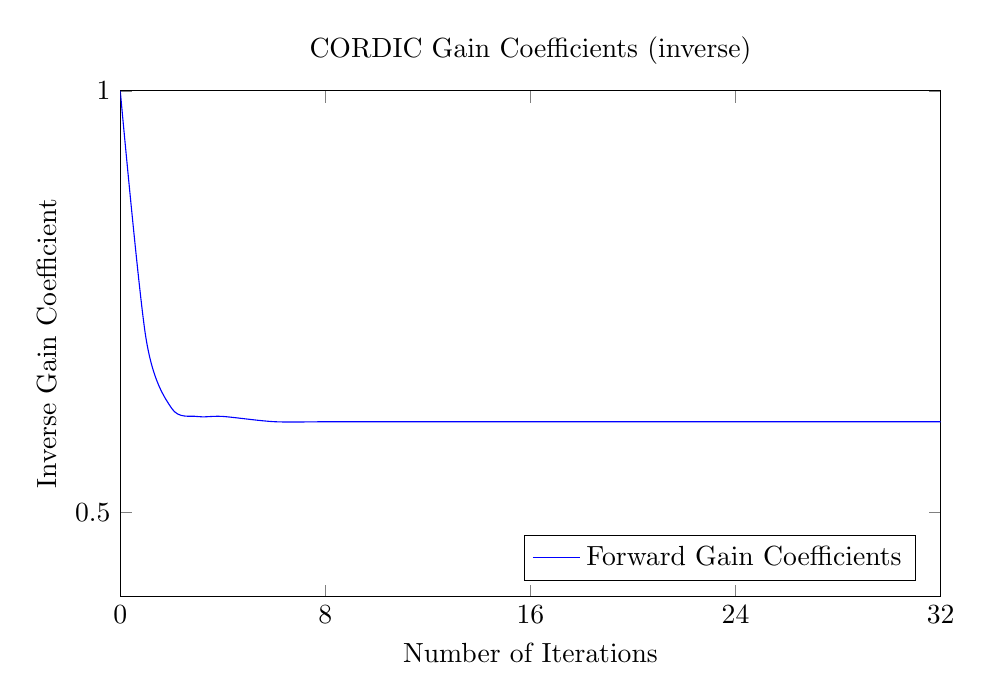
\begin{tikzpicture}

  \begin{axis}[    title={CORDIC Gain Coefficients (inverse)},    xlabel={Number of Iterations},    ylabel={Inverse Gain Coefficient},    xmin=0, xmax=32,    ymin=0.4, ymax=1,    xtick={0, 8, 16, 24, 32, 40, 48, 56, 64},    ytick={0, 0.5, 1, 1.5},    legend pos=south east,    grid style={dashed,gray!50},    width=12cm, height=8cm,    ]
    
    
    
    \addplot[
color=blue,
mark=,
smooth,
]
coordinates {
(0,1)
(1,0.7071)
(2,0.6234)
(3,0.6135)
(4, 0.6135719910778963)
(6, 0.6073517701412959)
(8, 0.607259112298892)
(10, 0.6072530315291342)
(20, 0.6072529350089730)
(32, 0.6072529350088808)
};
\legend{Forward Gain Coefficients, Inverse Gain Coefficients}
   \end{axis}

\end{tikzpicture}

   \label{CORDICcoeffPlot}
   \caption{Plot of CORDIC gain}
   
\end{center}

\end{figure}
\FloatBarrier

We observe a substantial convergence of the algorithm after approximately 8 iterations of the algorithm. The 8th iteration addresses rotations on the magnitude of $2^{-8}$, which is an extremely small rotation. Traditional \codeword{float} datatypes do not consider this level of precision.

\section{Optimization}
\end{document}